\section{Macros for the axes}

\tkzHandBomb\ Careful, these macros have been modified. It's now easier to use
the styles of \TIKZ. \tkzcname{tkzDrawX} allows to draw an axis,
\tkzcname{tkzLabelX} places graduations and finally in simple cases
\tkzcname{tkzAxeX} traces and graduations. The options of \TIKZ\ are accessible.
Fractions can be used for graduations.
%<--------------------------------------------------------------------->
%                  tkzDrawX
%<--------------------------------------------------------------------->
\subsection{\tkzcname{tkzDrawX}} \hypertarget{dx}{}

\begin{NewMacroBox}{tkzDrawX}{\oarg{local options}}%
This macro allows you to draw the abscissa axis with default ticks.
The options are those of \TIKZ\ plus the following ones:

\medskip
\begin{tabular}{lll}%
\toprule
options  & default & definition   \\
\midrule
\TOline{color}      {black}  {Axis and ticks}
\TOline{noticks}    {false}  {no ticks on axis}
\TOline{right space}{0.5 cm} {axis extended right}
\TOline{left space} {0 cm}   {extension of the axis to the left}
\TOline{label}      {$x$}    {label name}
\TOline{trig}       {0}      {if <>0 graduations are multiples of $pi$/trig"
"trig is an integer"}
\TOline{tickwd}     {0.8pt}  {tick thickness}
\TOline{tickup}     {1pt}    {tick over axis}
\TOline{tickdn}     {1pt}    {tick depth over axis}
\bottomrule
\end{tabular}

\medskip
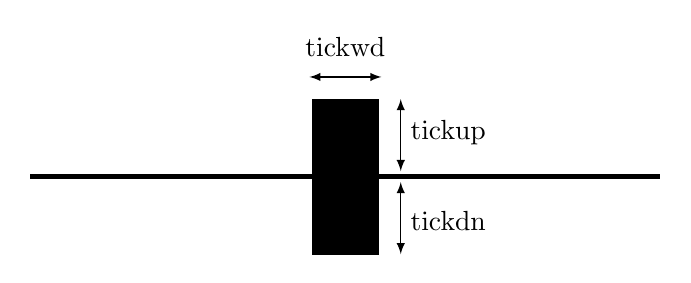
\begin{tikzpicture}[>=latex,scale=2]
  \draw[line width=2 pt](0,0)--(4,0);
  \draw[fill] (2cm-6pt,-14pt) rectangle (2cm+6pt,+14pt);
  \draw[<->](2cm-6.5pt,18pt) -- (2cm+6.5pt,+18pt);
  \node[above] at (2cm,20pt) {tickwd};
  \draw[<->](2cm+10pt,1pt) -- (2cm+10pt,+14pt);
  \node[right] at (2cm+10pt,8pt) {tickup};
  \draw[<->](2cm+10pt,-1pt) -- (2cm+10pt,-14pt);
  \node[right] at (2cm+10pt,-8pt) {tickdn};
\end{tikzpicture}

\medskip
This macro is used to draw the abscissa axis. The most important thing is to
test all the options. Above, you have the values that define a tick. Otherwise
the options of \TIKZ\ apply and in particular \tkzname{text}, \tkzname{color},
\tkzname{fill} and \tkzname{font}.
\end{NewMacroBox}

\subsubsection{No tick, no label}

\begin{tkzexample}[latex=8cm,small]
\begin{tikzpicture}
  \tkzInit[xmax=5]
  \tkzDrawX[label={},noticks]
\end{tikzpicture}
\end{tkzexample}

\subsubsection{Label placement}

\begin{tkzexample}[latex=8cm,small]
\begin{tikzpicture}
  \tkzInit[xmax=5]
  \tkzDrawX[label      = quantity,
            above left = 8pt]
\end{tikzpicture}
\end{tkzexample}

\subsubsection{Label and Axis Colour}

The color of the label is obtained with the option \tkzname{text}, that of the
axis with the option \tkzname{color}.

The option \tkzname{right=12pt} shifts the label $x$ by 12 pt.

\begin{tkzexample}[latex=7cm,small]
\begin{tikzpicture}
  \tkzInit[xmax=5]
  \tkzDrawX[text=blue,color=red,right=12pt]
\end{tikzpicture}
\end{tkzexample}

\subsubsection{Option \tkzname{right space}}

It adds a little space after the last tick.

\begin{tkzexample}[latex=6cm,small]
\begin{tikzpicture}
  \tkzInit[xmax=0.4,xstep=0.1]
  \tkzDrawX[text=blue,color=red,right=12pt,right space=1]
\end{tikzpicture}
\end{tkzexample}

\subsubsection{Trigonometric axis with the option \tkzname{trig=$n$}}\hypertarget{newm}{}

If $number=0$ then the axis is graduated from cm to cm, otherwise the axis is
graduated using multiples of $\frac{\pi}{number}$.

\begin{tkzexample}[latex=6cm,small]
\begin{tikzpicture}
  \tkzInit[xmin=0,xmax=4,ymin=-1,ymax=1]
  \tkzDrawX[trig=1]
\end{tikzpicture}
\end{tkzexample}

\subsubsection{Trigonometric axis with the option \tkzname{trig=2}}

\begin{tkzexample}[latex=6cm,small]
\begin{tikzpicture}
  \tkzInit[xmin=0,xmax=4,ymin=-1,ymax=1]
  \tkzDrawX[trig=2]
\end{tikzpicture}
\end{tkzexample}
%<--------------------------------------------------------------------->
%                  tkzLabelX
%<--------------------------------------------------------------------->
\subsection{\tkzcname{tkzLabelX}}\hypertarget{lx}{}

\begin{NewMacroBox}{tkzLabelX}{\oarg{local options}}%
This macro allows you to place graduations. The option \tkzname{orig} can be
used again, but its behavior is reversed. By default, the original value is
placed.
The options are those of \TIKZ, plus the following ones:

\medskip
\begin{tabular}{lll}
\toprule
options  & default & definition   \\
\midrule
\TOline{frac}  {0}{if <>0  graduations  are multiples num/frac "frac is an
integer"}
\TOline{trig}  {0}{if <>0  graduations are multiples $pi$/trig  "trig is an
integer"}
\TOline{font} {\BS textstyle} {scale size.}
\TOline{color}  {black} {graduation color}
\TOline{step}  {1} {interval between graduations}
\TOline{np off}  {false} {numprint deactivation}
\TOline{orig}  {true} {displays the origin graduation }
\bottomrule
\end{tabular}

{\tkzname{frac} and \tkzname{trig} are integers that can be changed to
fractional or trigonometric writing. }
\end{NewMacroBox}

\subsubsection{Position of the graduations}

\begin{tkzexample}[latex=6cm,small]
\begin{tikzpicture}
  \tkzInit[xmax=.5,xstep=0.1]
  \tkzDrawX[label=$t$,text=blue,color=red]
  \tkzLabelX[text=blue,below = 3pt]
\end{tikzpicture}
\end{tkzexample}

\subsubsection{Position of the graduations with \tkzname{xlabel style}}

\begin{tkzexample}[latex=5cm,small]
\begin{tikzpicture}
  \tkzInit[xmin=1000,xmax=4000,xstep=1000]
  \tkzDrawX
  \tikzset{xlabel style/.append style={rotate=-30}}
  \tkzLabelX[below right=3 pt,inner sep = 1pt]
\end{tikzpicture}
\end{tkzexample}

\subsubsection{Dates with \tkzname{np off}}

For dates, you have to deactivate numprint.
\begin{tkzexample}[latex=5cm,small]
\begin{tikzpicture}
  \tkzInit[xmin=2000,xmax=2004]
  \tkzDrawX
  \tikzset{xlabel style/.append style={rotate=-30}}
  \tkzLabelX[np off,below right=3 pt,inner sep =1pt]
\end{tikzpicture}
\end{tkzexample}

\subsubsection{\tkzname{frac}}

\begin{tkzexample}[latex=6cm,small]
\begin{tikzpicture}
  \tkzInit[xmax=1.75,xstep=0.33333]
  \tkzDrawX[label=$t$,text=blue,color=red]
  \tkzLabelX[frac=3,text=blue,below = 6pt]
  \end{tikzpicture}
\end{tkzexample}

\subsubsection{\tkzname{trig}}

\begin{tkzexample}[latex=6cm,small]
\begin{tikzpicture}
  \tkzInit[xmin=0,xmax=5,ymin=-1,ymax=1]
  \tkzDrawX[trig=2]
  \tkzLabelX[trig=2,text=blue,below = 8pt]
\end{tikzpicture}
\end{tkzexample}

\subsubsection{Graduations size}

Two possibilities. It is possible to define the default style used for the math
mode:

\begin{tkzltxexample}[small]
\let\tkzmathstyle\textstyle
\end{tkzltxexample}

\begin{tkzexample}[latex=6cm,small]
\begin{tikzpicture}
  \tkzInit[xmin=0,xmax=5,ymin=-1,ymax=1]
  \tkzDrawX[trig=2]
  \tkzLabelX[trig=2,text=blue,below = 8pt]
\end{tikzpicture}
\end{tkzexample}

\begin{tkzexample}[latex=6cm,small]
\begin{tikzpicture}
  \tkzInit[xmin=0,xmax=5,ymin=-1,ymax=1]
  \let\tkzmathstyle\textstyle
  \tkzDrawX[trig=2]
  \tkzLabelX[trig=2,text=blue,
            below = 8pt]
\end{tikzpicture}
\end{tkzexample}

\begin{tkzexample}[latex=6cm,small]
\begin{tikzpicture}
  \tkzInit[xmin=0,xmax=5,ymin=-1,ymax=1]
  \tkzDrawX[trig=2]
  \tkzLabelX[trig=2,text=blue,
           below = 8pt,node font=\small]
\end{tikzpicture}
\end{tkzexample}

\begin{tkzexample}[latex=6cm,small]
\begin{tikzpicture}
  \tkzInit[xmin=0,xmax=5,ymin=-1,ymax=1]
  \tkzDrawX[trig=2]
  \tkzLabelX[trig=2,text=blue,
      below = 8pt,node font=\scriptsize]
\end{tikzpicture}
\end{tkzexample}

\subsubsection{Colour of the graduations}

The key here is to use the color, text, and text options correctly.

\begin{tkzexample}[latex=7cm,small]
\begin{tikzpicture}
  \tkzInit[xmin = -2,xmax = 3,
           ymin = -2,ymax = 2]
  \tkzDrawX[color = red,
            label = $\displaystyle\frac{1}{t}$,
            below = 6pt]
  \tkzLabelX[text=blue]
\end{tikzpicture}
\end{tkzexample}

\subsubsection{Axis drawings before the graduation}

In some cases, it is preferable to place \tkzcname{tkzDrawXY} after
\tkzcname{tkzLabelX} and \tkzcname{tkzLabelY}.

This prevents display problems.

\begin{tkzexample}[latex=7cm,small]
\begin{tikzpicture}
  \tkzInit[xmin = -1,xmax = 4,
           ymin = -1,ymax = 1]
  \tkzDrawXY \tkzLabelX  \tkzLabelY
\end{tikzpicture}
\end{tkzexample}

\subsubsection{Graduations (except originally) prior to tracings}

\begin{tkzexample}[latex=7cm,small]
\begin{tikzpicture}
  \tkzInit[xmin = -1,xmax = 4,
           ymin = -1,ymax = 1]
  \tkzLabelX[orig=false]
  \tkzLabelY[orig=false]
  \tkzDrawXY
\end{tikzpicture}
\end{tkzexample}

\subsubsection{Only positive graduations before drawings}

\begin{tkzexample}[latex=7cm,small]
\begin{tikzpicture}
  \tkzInit[xmin=2,ymin=2,xmax=4,ymax=4]
  \tkzLabelX \tkzLabelY
  \tkzDrawXY
\end{tikzpicture}
\end{tkzexample}

\subsubsection{No graduations at the origin}

\begin{tkzexample}[latex=7cm,small]
\begin{tikzpicture}
  \tkzInit[xmin=2,ymin=2,xmax=4,ymax=4]
  \tkzLabelX[orig]    \tkzLabelY[orig]
  \tkzDrawXY
\end{tikzpicture}
\end{tkzexample}
%<--------------------------------------------------------------------->
%                  tkzAxeX
%<--------------------------------------------------------------------->
\subsection{\tkzcname{tkzAxeX}}\hypertarget{ax}{}

\begin{NewMacroBox}{tkzAxeX}{\oarg{local options}}%
This macro allows you to draw the abscissa axis with default ticks as well as
the graduations. It combines the two macros \tkzcname{tkzDrawX} and
\tkzcname{tkzLabelX}. It should only be used in simple cases.

\medskip
\begin{tabular}{lll}%
\toprule
options  & default & definition   \\
\midrule
\TOline{label} {$x$}{label name}
\TOline{trig} {0}{if <>0, graduations are multiples of $pi$/trig}
\TOline{frac} {0}{if <>0, graduations are multiples of 1/frac}
\TOline{swap} {false}{allows you to run \tkzcname{tkzLabelX} before
\tkzcname{tkzDrawX}}
\bottomrule
\end{tabular}

The option \tkzname{text} defines the color of the graduations.
\end{NewMacroBox}

\subsubsection{Example with \tkzcname{tkzAxeX}}
\begin{tkzexample}[latex=7cm,small]
\begin{tikzpicture}
  \tkzInit[xmax=0.5,xstep=0.1,ymax=1]
  \tkzGrid
  \tkzAxeX[text=blue]
\end{tikzpicture}
\end{tkzexample}

\subsubsection{Use of \tkzname{pi} and \tkzcname{tkzAxeX}}

\begin{tkzexample}[latex=5cm,small]
\begin{tikzpicture}
  \tkzInit[xmax=4,ymax=3.5]
  \let\tkzmathstyle\displaystyle
  \tkzLabelX[orig  = false, frac  = 4,below = 10pt]
  \tkzDrawX[label = $t$]
  \tkzAxeY[trig=2]
\end{tikzpicture}
\end{tkzexample}

\subsubsection{Option \tkzname{frac} and \tkzname{trig}}

In this example, we position the $t$ label as well as the graduations.
\tkzcname{below=10pt} is used to place the graduations underneath.

\begin{tkzexample}[latex=5cm,small]
\begin{tikzpicture}
  \tkzInit[xmax=9,xstep=3,ymax=3.5]
  \tkzLabelX[below=10pt,orig=false,frac=3]
  \tkzDrawX[label = $t$]
  \tkzAxeY[trig=2]
\end{tikzpicture}
\end{tkzexample}

%<--------------------------------------------------------------------->
%                  tkzDrawY
%<--------------------------------------------------------------------->
\subsection{\tkzcname{tkzDrawY}} \hypertarget{dy}{}

\begin{NewMacroBox}{tkzDrawY}{\oarg{local options}}%
This macro allows you to draw the ordinate axis with default ticks.
The options are those of \TIKZ\ plus the following ones:

\medskip
\begin{tabular}{lll}%
\toprule
options  & default & definition   \\
\midrule
\TOline{color}      {black} {color of axis and ticks}
\TOline{noticks}    {false} {no ticks on the axis}
\TOline{up space}   {0.5 cm} {top axis extension}
\TOline{down space} {0 cm}{axis extension down}
\TOline{label}      {$x$}{label name}
\TOline{trig}    {0}{if <>0, graduations are multiples of $pi$/trig "trig is an
integer" }
\TOline{tickwd}     {0.8pt}{tick's thickness}
\TOline{ticklt}     {1pt}{height of the tick above the axis}
\TOline{tickrt}     {1pt}{above-axis tick depth}
\end{tabular}
\end{NewMacroBox}

\subsection{\tkzcname{tkzLabelY}} \hypertarget{ly}{}

\begin{NewMacroBox}{tkzLabelY}{\oarg{local options}}%
This macro allows you to draw the abscissa axis with default ticks.
The options are those of \TIKZ\ plus the following ones:

\medskip
\begin{tabular}{lll}%
\toprule
options  & default & definition   \\
\midrule
\TOline{color}  {black} {graduation color}
\TOline{frac} {0}{if <>0, graduations are multiples of $1$/frac "frac is an
integer"}
\TOline{font} {\BS textstyle} {graduation size.}
\TOline{step}  {1} {interval between graduations}
\bottomrule
\end{tabular}

{\tkzname{frac} is a integer that can be changed to fractional or trigonometric
writing.}
\end{NewMacroBox}

%<--------------------------------------------------------------------->
%                  tkzAxeY
%<--------------------------------------------------------------------->
\subsection{\tkzcname{tkzAxeY}}\hypertarget{ay}{}
\begin{NewMacroBox}{tkzAxeY}{\oarg{local options}}%
This macro combines the two macros:
\tkzcname{tkzDrawY} \tkzcname{tkzLabelY}
See \tkzcname{tkzAxeX} for options.
\end{NewMacroBox}
%<--------------------------------------------------------------------->
%                  tkzAxeXY
%<--------------------------------------------------------------------->
\subsection{\tkzcname{tkzAxeXY}}  \hypertarget{axy}{}
\begin{NewMacroBox}{tkzAxeXY}{\oarg{local options}}%
This macro combines the four macros:
\tkzcname{tkzDrawX}\tkzcname{tkzDrawY} \tkzcname{tkzLabelX}\tkzcname{tkzLabelY}

It is necessary to use common options as in the example below, but this means
that the same options are applied to both macros. Thus it is not possible to
change \tkzname{label}.
\end{NewMacroBox}

\subsubsection{Colour of axes, graduations}

\begin{tkzexample}[latex=6cm]
\begin{tikzpicture}
  \tkzInit[xmin=-1,xmax=4,ymin=-1,ymax=3]
  \tkzAxeXY[label={},text=blue]
\end{tikzpicture}
\end{tkzexample}

\subsubsection{Option \tkzname{label=\{\}}}

\begin{tkzexample}[latex=6cm,small]
\begin{tikzpicture}
  \tkzInit[xmin=-1,xmax=4,ymin=-1,ymax=2]
  \tkzAxeXY[label={},text=blue,trig=2]
\end{tikzpicture}
\end{tkzexample}

\subsubsection{Option \tkzname{swap}}

\begin{tkzexample}[latex=6cm,small]
\begin{tikzpicture}
  \tkzInit[xmin=-2,xmax=2,ymin=-2,ymax=2]
  \tkzAxeXY[label={},swap]
\end{tikzpicture}
\end{tkzexample}
%<--------------------------------------------------------------------->
%                  tkzDrawXY
%<--------------------------------------------------------------------->
\subsection{\tkzcname{tkzDrawXY}}\hypertarget{dxy}{}

\begin{NewMacroBox}{tkzDrawXY}{\oarg{local options}}%
This macro combines the two macros: \tkzcname{tkzDrawX}\tkzcname{tkzDrawY}.
It is necessary to use common options as in the example below.
\end{NewMacroBox}

\subsubsection{Common colour and empty labels}
\begin{tkzexample}[latex=6cm,small]
\begin{tikzpicture}
  \tkzInit[xmin=-1,xmax=4,ymin=-1,ymax=1]
  \tkzDrawXY[label={},color=red]
\end{tikzpicture}
\end{tkzexample}

\subsubsection{Two trigonometric axes}

\begin{tkzexample}[latex=6cm,small]
\begin{tikzpicture}
  \tkzInit[xmin=-1,xmax=4,ymin=-1,ymax=1]
  \tkzDrawXY[label={},color=red,trig=4]
\end{tikzpicture}
\end{tkzexample}
%<--------------------------------------------------------------------->
%                  tkzLabelXY
%<--------------------------------------------------------------------->
\subsection{\tkzcname{tkzLabelXY}}  \hypertarget{lxy}{}

\begin{NewMacroBox}{tkzLabelXY}{\oarg{local options}}%
This macro combines the two macros:

\tkzcname{tkzLabelX}\tkzcname{tkzLabelY}

It is necessary to use common options as in the example below.
\end{NewMacroBox}

\subsubsection{}
\begin{tkzexample}[latex=6cm,small]
\begin{tikzpicture}
  \tkzInit[xmin=-1,xmax=4,ymin=-1,ymax=1]
  \tkzDrawXY[label={},color=red]
  \tkzLabelXY[text=blue]
\end{tikzpicture}
\end{tkzexample}

%<--------------------------------------------------------------------->
%                  tkzSetUpAxis
%<--------------------------------------------------------------------->
\subsection{Changing values by axis default} \hypertarget{axis}{}

\begin{NewMacroBox}{tkzSetUpAxis}{\oarg{local options}}%
\begin{tabular}{lll}%
options  & default & definition   \\
\midrule
\TOline{line width}{|0.4pt|}{line width defines the width of the line}
\TOline{tickwd}{|0.8pt|}{tick thickness  }
\TOline{ticka}{|1pt|}{right side or above the tick  }
\TOline{tickb}{|1pt|}{left side or below the tick  }
\TOline{font}{|\tkzcname{textstyle}|}{graduation size.}
\end{tabular}
\end{NewMacroBox}

\subsubsection{Changing the default axes}
\begin{tkzexample}[latex=5cm,small]
\begin{tikzpicture}[scale=1]
  \tkzInit[ymax=2,xmax=4]
  \tkzSetUpAxis[line width=1pt,tickwd=1pt,ticka=3pt, tickb=0pt]
  \tkzAxeXY
\end{tikzpicture}
\end{tkzexample}

You have to run \tkzcname{tkzSetUpAxis} again to retrieve the default values.

\medskip
\begin{tkzltxexample}[small]
\tkzSetUpAxis[line width=1pt,tickwd=1pt,ticka=2pt,tickb=2pt]
\end{tkzltxexample}

\tkzSetUpAxis[line width=1pt,tickwd=1pt,ticka=2pt,tickb=2pt]

\endinput
